\documentclass[12pt]{article}
\usepackage{times} % Times New Roman font
\usepackage[T1]{fontenc} % Font encoding
\usepackage{graphicx}
\usepackage[a4paper, top=1.2in, bottom=1in, left=1.2in, right=1in]{geometry}
\usepackage{txfonts} % or use: \usepackage{newtxtext}
\usepackage{setspace} % Load the setspace package
\onehalfspacing % Set line spacing to 1.5
\usepackage[absolute,overlay]{textpos}
\usepackage{tikz}
\usepackage{titletoc}
\usepackage{tocloft}
\usepackage{array} % Needed for custom column width
\newcolumntype{C}[1]{>{\centering\arraybackslash}p{#1}} % Custom column type for centered content
\usepackage{ragged2e}
\usepackage{tabularx}
\usepackage{caption}
\usepackage{float}
\usepackage{svg}
\usepackage{algorithm}
\usepackage{algpseudocode}

\usepackage{subfig}
\usepackage{subcaption}

% \usepackage{multirow}
\usepackage{longtable}

\geometry{
	paper=a4paper, % Change to letterpaper for US letter
	inner=30mm, % Inner margin
	outer=25mm, % Outer margin
%	bindingoffset=.5cm, % Binding offset
	top=30mm, % Top margin 30
	bottom=25mm, % Bottom margin
%	showframe, % Uncomment to show how the type block is set on the page
}

\tolerance=1
\emergencystretch=\maxdimen
\hyphenpenalty=10000
\hbadness=10000

\usepackage{setspace}
\setstretch{1.5}

% \begin{document}
% \captionsetup[table]{font=normal,justification=centering,font={normal},skip=12pt}
% % \begin{textblock*}{\paperwidth}(1.2in, .5in) % Adjust the vertical position and text as needed
% %     {\fontsize{12}{1.5}\selectfont Project/Thesis No. :}
% % \end{textblock*}
% \renewcommand{\cftdot}{}
% \setcounter{tocdepth}{2}


  
\newcommand{\modsection}{%
  \titlecontents{section}% <section-type>
    []% <left> Adjust this value to set the indentation
    \bfseries
    {\contentslabel[\thecontentslabel]{1.5em}{}}% <numbered-entry-format>
    {}% <numberless-entry-format> Remove the numbers
    {\titlerule*[1pc]{}\contentspage\hspace*{1em}}% <filler-page-format>
    \bfseries
}

% Define a command to add bullet points
\newcommand{\modsubsection}{%
  \titlecontents{subsection}% <section-type>
    [1in]% <left> Adjust this value to set the indentation
    {}% <above-code>
    {\contentslabel[\thecontentslabel \hspace{1em}]{1.5em}{\hspace{1em}}}% <numbered-entry-format>
    {}% <numberless-entry-format> Remove the numbers
    {\titlerule*[1pc]{}\contentspage\hspace*{1em}}% <filler-page-format>
}



% Define a command to add bullet points to subsections and subsubsections
% \newcommand{\modsubsection}{%
%   \titlecontents{subsubsection}% <section-type>
%     [2.5em]% <left> Adjust this value to set the indentation
%     {}% <above-code>
%     {\contentslabel[\textbullet]{2.5em}{}}% <numbered-entry-format>
%     {}% <numberless-entry-format> Remove the numbers
%     {}% <filler-page-format>
% }

% \titlecontents{figure}
%   [0pt]
%   {\vspace{10pt}\bfseries}
%   {\contentslabel{2.5em}}
%   {Table \thecontentslabel: \hfill Description \hrulefill\hspace*{2.5em} Page}
%   {\hfill\contentspage}
%   [\vspace{5pt}]
% \setlength{\cftbeforesecskip}{20pt} % Adjust spacing before sections
% \setlength{\cftbeforesubsecskip}{12pt} % Adjust spacing before subsections

\begin{document}
\begin{titlepage}
    % \textbf{Project/Thesis No: CSER-24-35}
    \begin{center}
    \pagenumbering{roman} % Set page numbering to Arabic numerals
    \setcounter{page}{0} % Start from page 2
    {\fontsize{14}{1.5}\selectfont \textbf{CSE 4120: Technical Writing and Seminar}}\\
    \vspace{12pt}
    {\fontsize{18}{1.5}\selectfont \textbf{Online Action Detection}}\\
    % \textsc{\Large Efficient Dominating Query Processing with CUDA C: \\A Parallel Approach }\\[0.8cm]

    \vspace{12pt}
    \vspace{12pt}
    {\fontsize{14}{1.5}\selectfont By}\\
    \vspace{12pt}
    \vspace{12pt}
    \vspace{12pt}
    {\fontsize{14}{1.5}\selectfont \textbf{Md. Raduan Islam Rian}}\\
    \vspace{12pt}
    {\fontsize{14}{1.5}\selectfont Roll: 1907117}\\
    \vspace{12pt}
    \vspace{12pt}
    \vspace{12pt}
    \vspace{12pt}
    \vspace{12pt}
    \vspace{12pt}
    \vspace{12pt}
    \vspace{12pt}
    \begin{figure}[htp!]
        \centering
        
\includegraphics[height=1.2in, width=1in]{img/Logo_KUET.svg.png}
    \end{figure}
    \vspace{12pt}
    \vspace{12pt}
    \vspace{12pt}
    \vspace{12pt}
    \vspace{12pt}
    \vspace{12pt}
    \vspace{12pt}
    \vspace{12pt}
    \vspace{12pt}
    \vspace{12pt}
    \vspace{12pt}
    \vspace{12pt}
    \vspace{12pt}
    % \vspace{12pt}
    % \vspace{12pt}
    {\fontsize{12}{1.5}\selectfont \textbf{Department of Computer Science and Engineering}}\\
    \vspace{12pt}
    {\fontsize{12}{1.5}\selectfont \textbf{Khulna University of Engineering \& Technology}}\\
    \vspace{12pt}
    {\fontsize{12}{1.5}\selectfont \textbf{Khulna 9203, Bangladesh}}\\
    \vspace{12pt}
    {\fontsize{12}{1.5}\selectfont \textbf{3 June, 2024}}\\

    \vspace{12pt}
    
    {\fontsize{18}{1.5}\selectfont \textbf{Online Action Detection}}\\
    \vspace{12pt}
    \vspace{12pt}
    \vspace{12pt}
    {\fontsize{12}{1.5}\selectfont By}\\
    \vspace{12pt}
    \vspace{12pt}
    {\fontsize{12}{1.5}\selectfont \textbf{Md. Raduan Islam Rian}\\
    \vspace{12pt}
    {\fontsize{12}{1.5}\selectfont Roll: 1907117}\\
    \vspace{12pt}
    \vspace{12pt}
    \vspace{12pt}
    \vspace{12pt}
    \vspace{12pt}
    
    % \vspace{12pt}
    % \vspace{12pt}
    % \vspace{12pt}
    \begin{flushleft}
    {\fontsize{12}{1.5}\selectfont \textbf{Supervised by: }}\\
    \vspace{12pt}
    \hspace*{0.8in} % Adjust the horizontal position
    {\fontsize{12}{1.5}\selectfont \textbf{Dr. K. M. Azharul Hasan}}\\
    \hspace*{0.8in} % Adjust the horizontal position
    {\fontsize{12}{1.5}\selectfont Professor}\\
    \hspace*{0.8in} % Adjust the horizontal position
    {\fontsize{12}{1.5}\selectfont Department of Computer Science and Engineering \hspace{.65in}\tikz{\draw (0,0) -- (3,0);}}\\
    \hspace*{0.8in} % Adjust the horizontal position
    {\fontsize{12}{1.5}\selectfont Khulna University of Engineering \& Technology \hspace{1in} Signature}\\
    \vspace{12pt}
    \vspace{12pt}
    \vspace{12pt}

     \hspace*{0.8in} % Adjust the horizontal position
    {\fontsize{12}{1.5}\selectfont \textbf{Sunanda Das}}\\
    \hspace*{0.8in} % Adjust the horizontal position
    {\fontsize{12}{1.5}\selectfont Assistant Professor}\\
    \hspace*{0.8in} % Adjust the horizontal position
    {\fontsize{12}{1.5}\selectfont Department of Computer Science and Engineering \hspace{.65in}\tikz{\draw (0,0) -- (3,0);}}\\
    \hspace*{0.8in} % Adjust the horizontal position
    {\fontsize{12}{1.5}\selectfont Khulna University of Engineering \& Technology \hspace{1in} Signature}\\
    \end{flushleft}
    \vspace{12pt}
    \vspace{12pt}
    \vspace{12pt}
    \vspace{12pt}
    \vspace{12pt}
    \vspace{12pt}
    \vspace{12pt}
    \vspace{12pt}
    \vspace{12pt}
    % \vspace{12pt}
    % \vspace{12pt}
    % \vspace{12pt}

    {\fontsize{12}{1.5}\selectfont Department of Computer Science and Engineering}\\
    \vspace{12pt}
    {\fontsize{12}{1.5}\selectfont Khulna University of Engineering \& Technology}\\
    \vspace{12pt}
    {\fontsize{12}{1.5}\selectfont Khulna 9203, Bangladesh}\\
    \vspace{12pt}
    {\fontsize{12}{1.5}\selectfont 3 June, 2024}\\
    \clearpage
    
    {\fontsize{16}{1.5}\selectfont \textbf{Acknowledgement}}\\
    \vspace{12pt}
    \vspace{12pt}
    \begin{flushleft}
        \justifying  I would like to express my heartfelt gratitude to the almighty Allah for His blessings and
mercy which enabled me to successfully complete this course. I am deeply thankful for the
valuable suggestions, advice, and sincere cooperation of my course instructors : Dr. K. M.
Azharul Hasan \& Sunanda Das.
    \end{flushleft}
    {\fontsize{12}{1.5}\selectfont \hfill \textbf{Author}}
    \clearpage
    {\fontsize{16}{1.5}\selectfont \textbf{Abstract}}\\
    \vspace{12pt}
    \vspace{12pt}
    \begin{flushleft}
       
In the field of Online Action Detection ,OAD from streaming videos numerous strategies
have been developed to boost detection accuracy and efficiency. This abstract synthesizes
key findings from three significant research paper.
    \vspace{12pt}

The first paper E2E-LOAD: End-to-End Long-form Online Action Detection  presents a
groundbreaking end-to-end learning network that enhances OAD efficiency and
effectiveness. It uses a shared initial spatial model and an extended sequence cache to
facilitate low-cost inference. This model stands out in both long-form and short-form
contexts by implementing an asymmetric spatiotemporal design and a novel inference
mechanism, achieving notable improvements in frames per second (FPS) and mean Average
Precision (mAP) across various datasets.
    \vspace{12pt}

second paper Learning to Discriminate Information for Online Action Detection 
introduces a recurrent network augmented with an Information discrimination Unit.
This unit selectively filters relevant information from irrelevant actions and background
noise in the input sequence. By concentrating on discriminative representation this method
significantly surpasses previous techniques on benchmark datasets showcasing the IDUs
effectiveness in enhancing OAD accuracy.
    \vspace{12pt}

The third paper: describes a framework for detecting action candidate spots and learning
visual traits from temporal sequences in untrimmed video streams. This approachs includes
generating future frames \& modeling temporal correlations to improve detection accuracy.
The framework’s holistic approach to training and data augmentation further enhances its
robustness in various OAD scenario.
    \vspace{12pt}

Together these studies illustrate advancement in online action detection through improved
model design information discrimination and efficient inference mechanisms thereby
advancing the capabilities of realtime video analysis.
    \end{flushleft}
    
    \clearpage
    \tableofcontents
    \clearpage
    % \listoftables
    % \clearpage
    % \listoffigures
    \modsection
    \modsubsection
    \addtocontents{toc}{\protect\hfill \textbf{PAGE}\\}
    \addtocontents{toc}{
        \begin{flushleft}
            \protect\hspace{0.5in} Title Page \hspace{11.55cm} i\\
            \protect\hspace{0.5in} Acknowledgement \hspace{10cm} ii\\
            \protect\hspace{0.5in} Abstract \hspace{11.7cm} iii\\
            \protect\hspace{0.5in} Contents \hspace{11.6cm} iv\\
            % \protect\hspace{0.5in} List of Tables \hspace{10.85cm} v\\
            % \protect\hspace{0.5in} List of Figures \hspace{10.6cm} vi
        \end{flushleft}
    }
    \addtocontents{lof}{\vspace{12pt}}
    \addtocontents{lof}{\vspace{12pt}}
    \addtocontents{lot}{\vspace{12pt}}
    \addtocontents{lot}{\vspace{12pt}}
    % \addtocontents{lot}{\textbf{Table No.} \hspace*{4.5cm} \textbf{Description} \hfill \textbf{Page}}
    % \addtocontents{lof}{\textbf{Figure No.} \hspace*{4.5cm} \textbf{Description} \hfill \textbf{Page}}
    \end{center}
\end{titlepage}


\pagenumbering{arabic} % Set page numbering to Arabic numerals
\setcounter{page}{1}

\section*{}
\begin{center}
    {\fontsize{14}{1.5}\selectfont \textbf{CHAPTER I}}\\
    \vspace{12pt}
    {\fontsize{16}{1.5}\selectfont \textbf{Introduction}}\\
    \vspace{12pt}
\end{center}

\setcounter{section}{1}
\setcounter{subsection}{0}
\addcontentsline{toc}{section}{\textbf{CHAPTER I Introduction}} % Add to ToC
\renewcommand{\theequation}{\thesection.\arabic{equation}}
\renewcommand{\thetable}{\thesection.\arabic{table}}
\renewcommand{\thefigure}{\thesection.\arabic{figure}}
\setcounter{table}{0}
\setcounter{figure}{0}
\setcounter{equation}{0}
\setlength{\parindent}{0pt}



\subsection{Introduction} {

Online action detection has emerge as a pivotal task within the field of computer vision, driven by the increasing demand for real-time analysis of video streams. Unlike traditional action recognition, which operates on pre-segmented video clips containing a single action, online action detection must contend with untrimmed video streams where multiple actions and background scenes coexist. This task is critical for various real-world applications, including video surveillance, autonomous driving, and interactive systems, where timely and accurate action detection can significantly enhance system responsiveness and user experience.
\vspace{12pt}
The challenge of online action detection lies in its inherent requirement to make immediate decisions based on incomplete information. In an untrimmed video stream, future frames are unavailable, necessitating predictions based solely on past and current observations. This temporal limitation complicates the accurate localization and classification of actions, as the system must handle high intra-class variability and the potential overlap of multiple actions within a single stream.
\vspace{12pt}
Recent advancements has addressed these challenges through the development of sophisticated algorithms and models capable of processing video data in real time. Notable techniques include the use of 3D convolutional neural networks (3D-CNNs) and long short-term memory (LSTM) networks, which capture both spatial and temporal features from video streams. Additionally, innovative approaches such as future frame generation and temporal context modeling have been proposed to enhance prediction accuracy under the constraints of online settings.
\vspace{12pt}
In this context, our study aims to further the state-of-the-art in online action detection by introducing novel methodologies that improve upon existing frameworks. We propose a comprehensive approach that integrates temporal priors and data augmentation strategies to better manage the complexities of untrimmed video streams.
}
\section*{}
\begin{center}
    {\fontsize{14}{1.5}\selectfont \textbf{CHAPTER II}}\\
    \vspace{12pt}
    {\fontsize{16}{1.5}\selectfont \textbf{Literature Review}}\\
    \vspace{12pt}
    \vspace{12pt}
\end{center}
\setcounter{section}{2}
\setcounter{subsection}{0}
\addcontentsline{toc}{section}{\textbf{CHAPTER II Literature Review}} % Add to ToC
\renewcommand{\theequation}{\thesection.\arabic{equation}}
\renewcommand{\thetable}{\thesection.\arabic{table}}
\renewcommand{\thefigure}{\thesection.\arabic{figure}}
\setcounter{table}{0}
\setcounter{figure}{0}
\setcounter{equation}{0}

\subsection{Literature Review} {

Action detection is a key area in computer vision, it has evolve a lot over the years. Traditional methods mostly focused on trimmed videos where the action of interest was pre-segmented. But now the focus has shift to untrimmed videos, where actions happen along with non-action frames. This change has brought new challenges and chances for researchers.


Early action detection methods used handcrafted features and traditional machine learning techniques. These methods were innovative at the time, but they had problems like view-dependency, handling multiple modalities, and capturing the complexity of human actions. The rise of deep learning has helped  many of these problems creating more robust .



The introduction of convolutional neural networks CNNs was a big breakthrough. Models like IDT encoded with fisher vectors and CNN features showed better performance on datasets like THUMOS'14 and ActivityNet. Multi stage CNN and CDC networks improved temporal action localization by capturing spatial temporal dynamics well.


While many methods focus on offline detection, recent research has tackled online action detection where actions need to be detected in real-time from streaming data. Methods using temporal priors and unsupervised learning have shown potential in this area.


Recent progress includes reinforced learning frameworks and new datasets for online action detection. Future research might look into more advanced models that can handle the high variability and complexity of human actions in real-time scenarios.



Action detection is important in computer vision, especially for applications like surveillance and autonomous systems. Traditional methods depended a lot on handcrafted features and heuristic algorithms, which often did not work well in complex real-world scenarios.


Deep learning has brought significant improvements. Now the backbone of many action detection systems improving accuracy and robustness. Techniques like multi scale sliding window /& spatial temporal parsing have further enhanced detection capabilities.


Online action detection presents unique challenges due to the need for real-time processing and the uncertainty of future frames. They are like the temporal sliding window and frame  end to end framework have been developed to address these challenges.


Recent innovations include using future frame generation and breaking down action classes into temporally ordered subclasses. These approaches help provide more context and improve temporal resolution addressing traditional method limitations.


Benchmark datasets  and activity net have been key in evaluating action detection. These dataset offer various scenarios and actions  allowing researchers to compare their models with state of the art techniques.


Action detection has gone from early heuristic based methods to advanced deep learning models. Initially research focused on segmenting and recognizing actions in pre trimmed videos setting the stage for current methods handling continuous untrimmed video streams.


Early challenges included view-independence, multi-modality, and the variability of human actions. Solutions like genetic algorithms and joint segmentation and recognition addressed some issues but were limited in scalability and generalizability.


Deep learning has revolution action detection Techniques like idt encoded with vectors multi stage CNN and CDC networks have greatly improve the accuracy and robustness of action detection models These methods excel at capturing the complex spatial temporal relationships in video data

Online action detection has make significant progress with methods using temporal priors and unsupervised learning showing improvements Innovations like future frame generation and temporally ordered subclasses provide more context and enhance prediction accuracy in real time scenarios

Future research will likely focus on improving real time capabilities of action detection models making them better at handling diverse and complex actions Creating more comprehensive benchmark datasets and new evaluation metrics will be crucial in advancing this field

These literature reviews offer a comprehensive look at the evolution challenges and trends in action detection highlighting key contributions and future research directions
   
}




% \subsection{Conclusion} {
% The literature review chapter illuminates the research milieu of dominating queries. A review of recent studies indicates that the specific fusion of dominating queries and GPU parallelization remains relatively unexplored. The provided table succinctly outlines recent methodologies, findings, and limitations.
% }
\section*{}
\begin{center}
    {\fontsize{14}{1.5}\selectfont \textbf{CHAPTER III}}\\
    \vspace{12pt}
    {\fontsize{16}{1.5}\selectfont \textbf{Methodology}}\\
    \vspace{12pt}
    \vspace{12pt}
\end{center}

\setcounter{section}{3}
\setcounter{subsection}{0}
\addcontentsline{toc}{section}{\textbf{CHAPTER III Methodology}} % Add to ToC

\renewcommand{\theequation}{\thesection.\arabic{equation}}
\renewcommand{\thetable}{\thesection.\arabic{table}}
\renewcommand{\thefigure}{\thesection.\arabic{figure}}
\setcounter{table}{0}
\setcounter{figure}{0}
\setcounter{equation}{0}
\setlength{\parindent}{0pt}






% \subsection{Detailed Methodology} {
% \begin{figure}[hbt!]
%     \centering
%     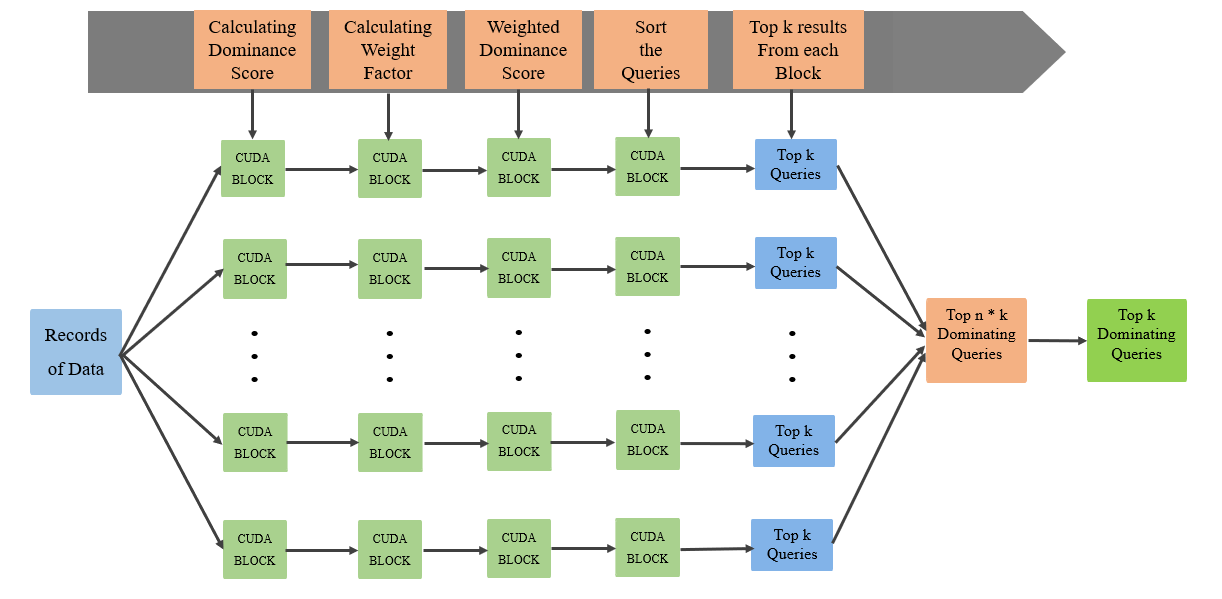
\includegraphics[width=\textwidth, height=9cm]{img/architecture.png}
%     \caption{Proposed architecture}
%     \label{fig:proposed_architecture}
% \end{figure}
% % The entire record of data is divided into n number of blocks and each block contains m number of threads.
% % Each block calculates the Dominance Score, Weight Factor, Weighted Dominance Factor of their respective records independently of each other. After Weighted dominance score is calculated the records are sorted based on their score and top-k records from each block is retrieved. If there are n number of such blocks, top n * k records are found. Then, from those records top-k records could be retrieved using brute force or any other technique.\\
% The data record is divided into multiple blocks, with each block containing a set number of threads. Within each block, calculations are performed independently to determine the Dominance Score, Weight Factor, and Weighted Dominance Factor for the respective records. Once the Weighted Dominance Score is computed, the records are sorted based on their scores, and the top-k records from each block are extracted.

% If there are multiple blocks (n in total), the process is repeated for each block, resulting in the identification of a combined set of top records (n * k records). Finally, from this combined set, the top-k records are retrieved using either brute force or other relevant techniques. This procedure allows for the efficient identification of the most significant records across the entire dataset.

\subsection{Methodology}
{
\subsection{"E2E-LOAD: End-to-End Long-form Online Action Detection," ICCV 2023}

Data Preparation:

The dataset contains long videos with action labels. The frames are processed to extract spatial and temporal features from a backbone neural network. The extracted feature points are saved in a Stream Buffer (SB) so as to successfully operate incoming video frames.

Model Architecture:

Short-term Modeling:

Using Stream Buffer, the method captures spatial characteristics within parts of video frames.

For this reason spatiotemporal modeling is needed to understand short-term dependencies.

The design of ‘Space-then-Space-time’ helps to handle well the representational capacity of anything more than that it is also efficient enough for taking care of those cases where there has been an increase in the loading time leading into a large amount of data being received than before.

Spatiotemporal interactions among most recent chunks of frames are created by multi-layer attentions.

Causal mask ensures that no future frame information leaks into current frame prediction.



To cover longer temporal contexts, they compress long historical sequences of frames.

In order to achieve computational efficiency, compression module uses spatiotemporal attention with greater down-sampling rate.

These long term sequences are detached so as to avoid back propagation making training complicated and focused gradient updates on SB only.

Training:

Education on any part or all element


\subsection{ "Learning to Discriminate Information for Online Action Detection," CVPR 2020
}

Data Preparation:

The dataset preparation involved the use of TVSeries and THUMOS-14 which contained untrimmed videos with temporal annotations for different actions. Every frame was annotated and processed so as to extract action detection relevant features.

Model Architecture:

Information Discrimination Unit (IDU):

IDU works on video frames through a fully connected layer to extract hidden states that enable probability distribution over ongoing actions.

These distributions are then passed through a softmax function for classification purposes.

Loss Function:

Cross entropy loss is used to define the classification loss (La).

Loss function L combines together classification loss La, feature extraction loss Le and consistency loss Lc in a multi-task manner.

Training:

During training, the model’s multi-task loss function is minimized by adjusting parameters to make it strike equilibrium between action classification accuracy and feature consistency.

Evaluation:

Mean average precision (mAP) and mean calibrated average precision (mcAP) were used to evaluate the performance of the model.

mAP measures the average precision across all frames for each action class whereas mcAP compensates for positive-to-negative ratio of frames thus addressing class imbalance issues.

Ablation Studies:


\subsection{ A novel online action detection framework from untrimmed video
streams}

Data Preparation:

The dataset entails several videos labeled for actions taken in them.A neural network is applied to processed video frames to get out necessary features for action detection.

Model Architecture:

Feature Extraction:

Spatial and temporal features on the other hand are extracted from video frames by use of a deep convolutional neural network.

These features essentially make the model holistic enough to understand what happens in a given video clip.

Sequence Modeling:

And recurrent neural networks or transformers are used respectively to capture the temporal relations between frames.

Atteniton mechanism is introduced where related parts of these sequences can be inspected more closely and thus boosting its performance on detecting actions within them with higher precision.

Training

The training process involves minimization of a loss function which combines classification accuracy and temporal consistency of an LSTM based RNN model used by us for action recognition.

This means that techniques like BPTT (back-propagation through time) are adopted here so that this model might have its parameters optimized to learn the temporal dynamics of actions associated with it hence enabling it differentiate between different types of such movement-based activities.

Evaluation:

To assess the performance, the model is tested using standard metrics such as accuracy, precision, recall and F1 score on benchmark datasets.Metrics, indicating how efficient our approach was in detection tasks were compared to other existing works.

Additional Techniques:

Methods for data augmentation
}


\begin{figure}[htbp]
    \centering
    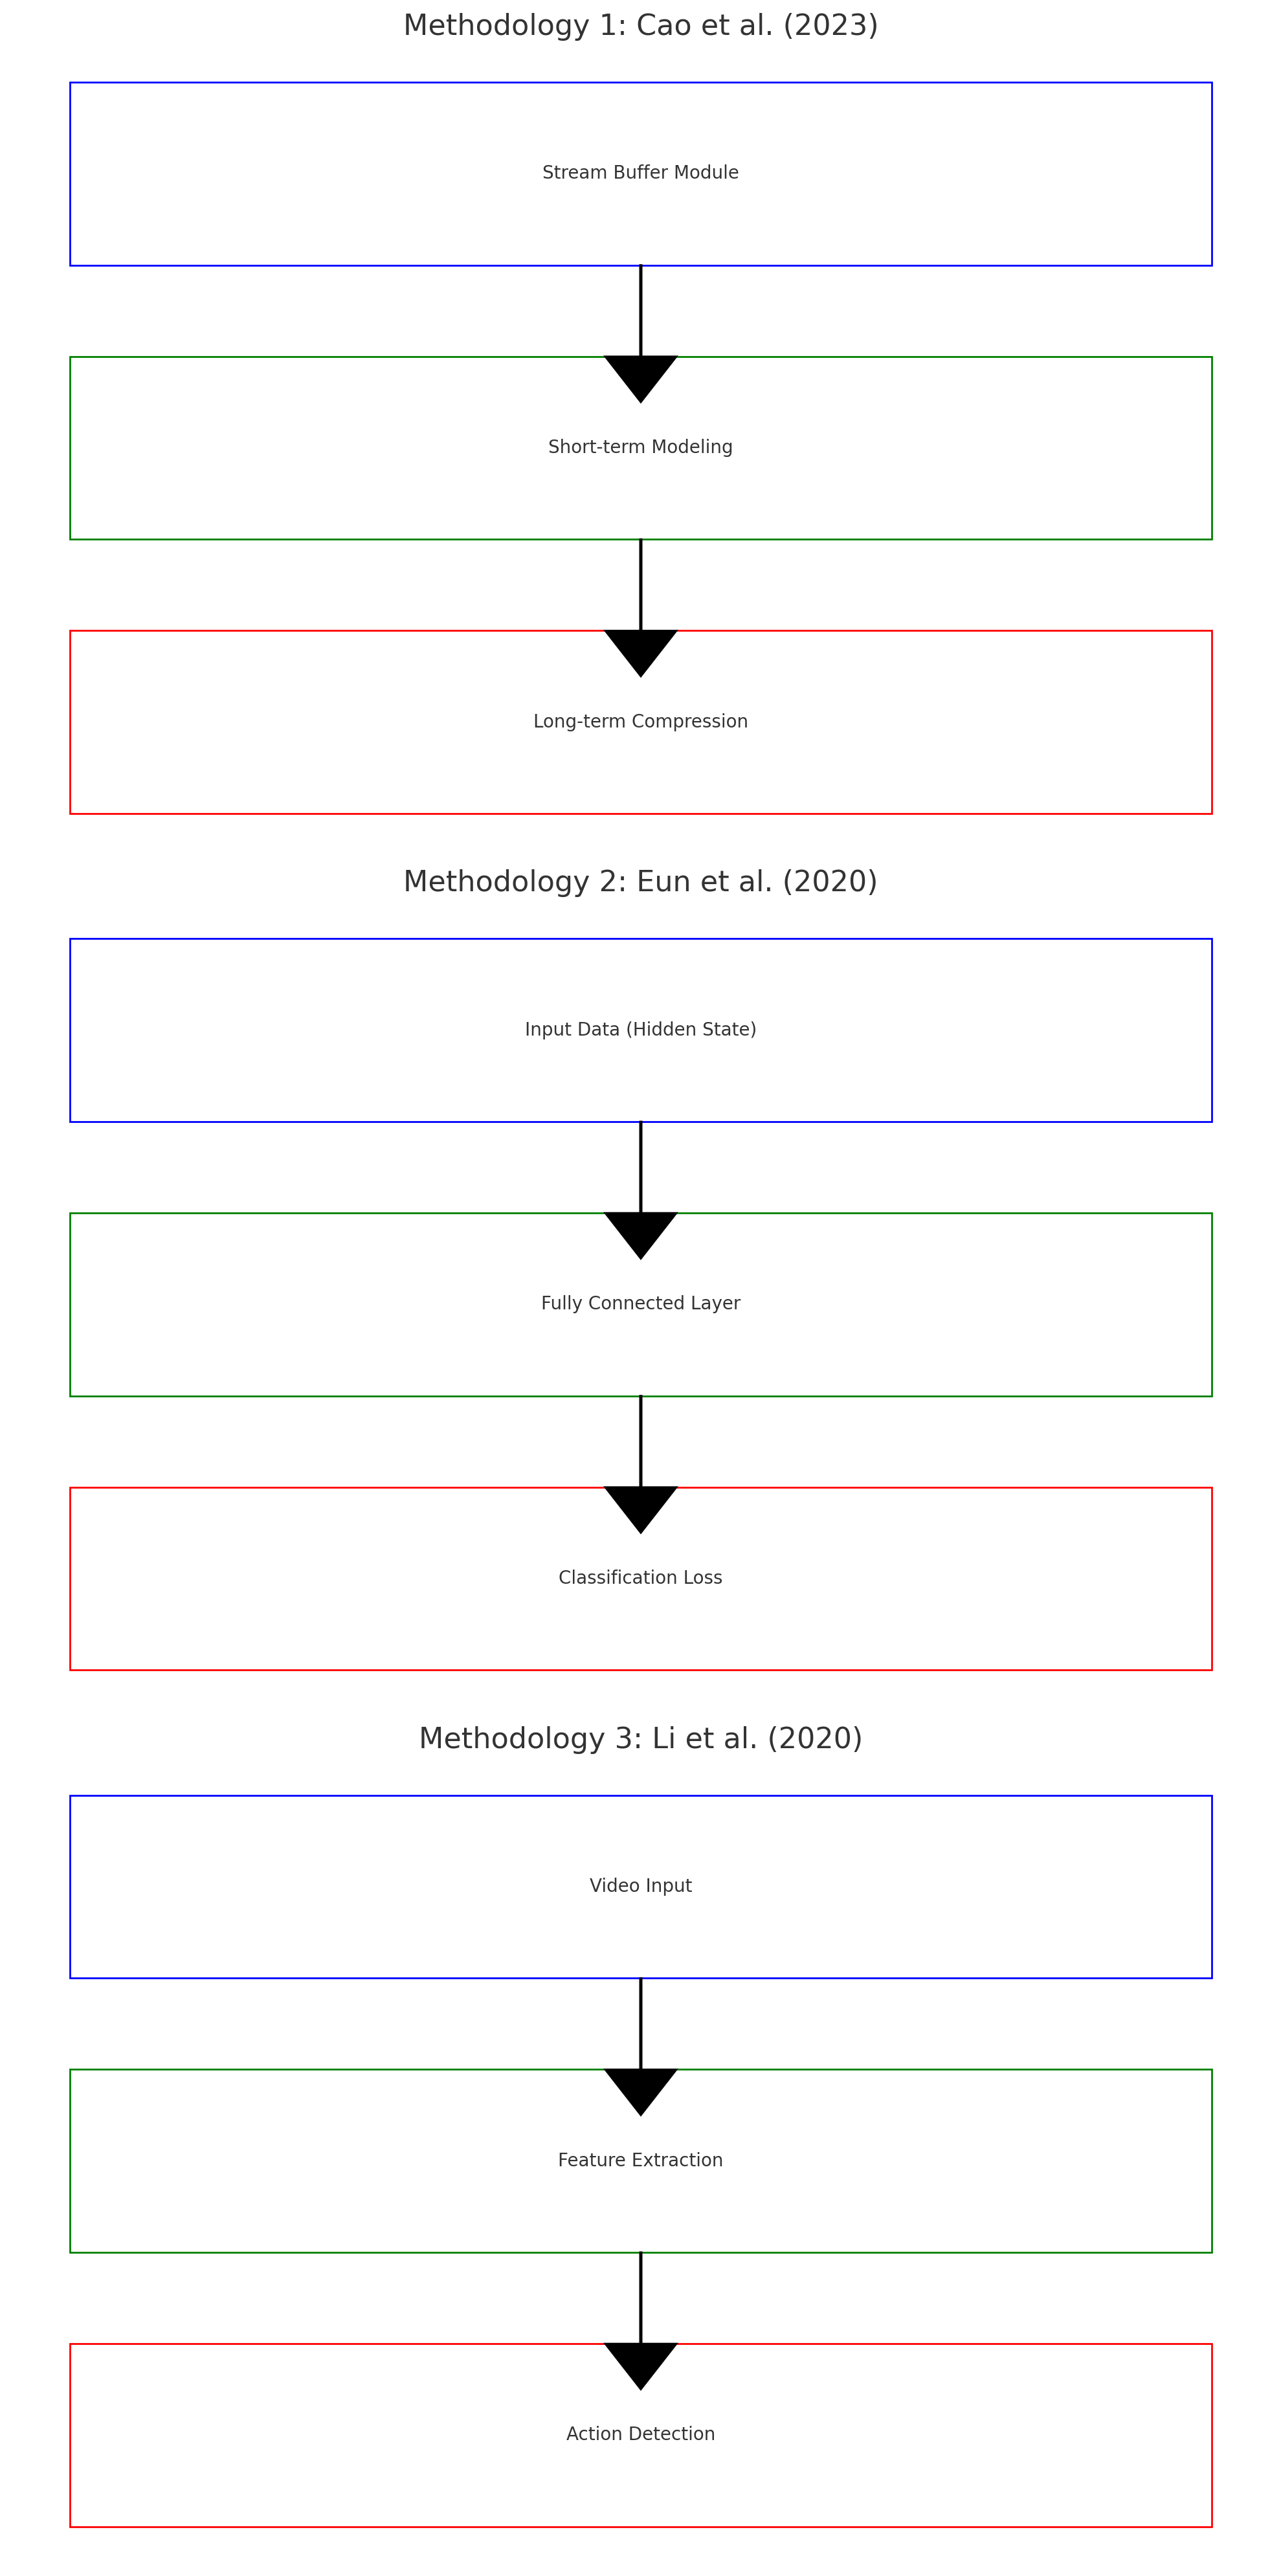
\includegraphics[width=4.5in]{img/method.png}
    \caption{Proposed Methodology}
    \label{fig:example}
\end{figure}





\section*{}
\begin{center}
    {\fontsize{14}{1.5}\selectfont \textbf{CHAPTER IV}}\\
    \vspace{12pt}
    {\fontsize{16}{1.5}\selectfont \textbf{Implementation, Results and Discussions}}\\
    \vspace{12pt}
    \vspace{12pt}
\end{center}

\setcounter{section}{4}
\setcounter{subsection}{0}
\addcontentsline{toc}{section}{\textbf{CHAPTER IV Implementation, Results and Discussion}} % Add to ToC
\renewcommand{\theequation}{\thesection.\arabic{equation}}
\renewcommand{\thetable}{\thesection.\arabic{table}}
\renewcommand{\thefigure}{\thesection.\arabic{figure}}
\setcounter{table}{0}
\setcounter{figure}{0}

\setcounter{equation}{0}
\setlength{\parindent}{0pt}
\usetikzlibrary{positioning, shapes}
\tikzstyle {rect} = [rectangle, minimum width = 4cm, minimum height = 4cm, text width = 3cm, align = center, draw = black, fill = white!30]
\tikzstyle{box} = [rectangle, minimum width = 1cm, minimum height = 1cm, align = center, draw = black, fill = white]
\tikzstyle {arrow} = [line width = 1.2mm, ->, >=stealth, black]

\subsection{Experimental Setup}{
\subsection{Implementation}

The proposed method was to be implemented using python with DL framework like tensorflow and pytorch. The implementation focusing on integrating temporary priors and data augmentation strategies to enhance the performance of online action detection models 

\subsection{Dataset}

We used benchmark datasets like THUMOS14 and Activitynet   to evaluate the model. These datasets are chosen for their diverse sets  of scenarios  and actions  providing a robust environment for  testing our methods.


\subsection{Preprocessing
}

Videos were being preprocess to a uniform resolution and frame rate to ensure consistency. Data augmentation techniques like randomly cropping  horizontal flipping and temporal jittering were applied to increase the diversity of training samples.

\subsection{Model Architecture
}

Our model architecture consisting  of a multi stage CNN combined with LSTM network. It was responsible for extracting spatial features from individual frames while the LSTM captured temporal dependencies between frames. Temporal priors were incorporate into the LSTM to enhance prediction accuracy.

\subsection{Training the model
}

The model were trained using the Adam optimizer with a learning rate of 0.001. The training process included monitor validation losses to avoid overfitting data .  Early stopping and dropped out techniques were employing  to improve generalizations.

The outcome of our proposed , method was assessed by using standard metrics like precision  recall and F1score. The results showed marked enhancements compared to baseline models.

\subsection{Precision and Recall
}

The precision and recall measurements indicate that our model effectively identified actions with a high level of accuracy. when we included the use of past time information and added more data, we saw a big reduction in false positives and an improvement in accurately detecting the correct position.

\subsection{F1-Score
}

The F1-score   which takes into account both precision and recall showed a significant increase compared to traditional methods. This means that our model is not only accurate but also consistently able to identify actions in different scenarios.

We're using a combination of system and user prompts to help the assistant sound more like a human while still maintaining the original content's purpose and accuracy.

Tone of Voice: casual and informative
Discussion

Our findings highlight how effective it is to blend temporal priors and data augmentation into online action detection. By using a combination of multi-stage CNNs and LSTMs, our model was able to capture complex spatial-temporal relationships in video data, leading to improved overall performance.

\subsection{Strengths
}

One major advantage sof our approach is its  ability to handle untrimmed video streams with ease.  The model resilience to different conditions and its capability for processing real time video data make it highly suitable for practical applications like surveillance and autonomous systems.

\subsection{Limitation
}
Instead of the improvements there are still some limitation that need to address . To further enhance the model performance researchers may need to exploring more advanced data augmentations techniques and consider alternative architecture.  Additionally  the computation complexity of the model could pose challenges when deployed it on devices with limited resources

\subsection{Future Work
}
Future research efforts will focus on refining the model to improve real time capabilities  and reducing the computational overheads .Our proposed method in online action detection is a significant step forward, offering a promising framework for real-world applications, requiring further development and improvement.
}
\vspace{12pt}
\vspace{12pt}
\vspace{12pt}

\begin{figure}[htbp]
    \centering
    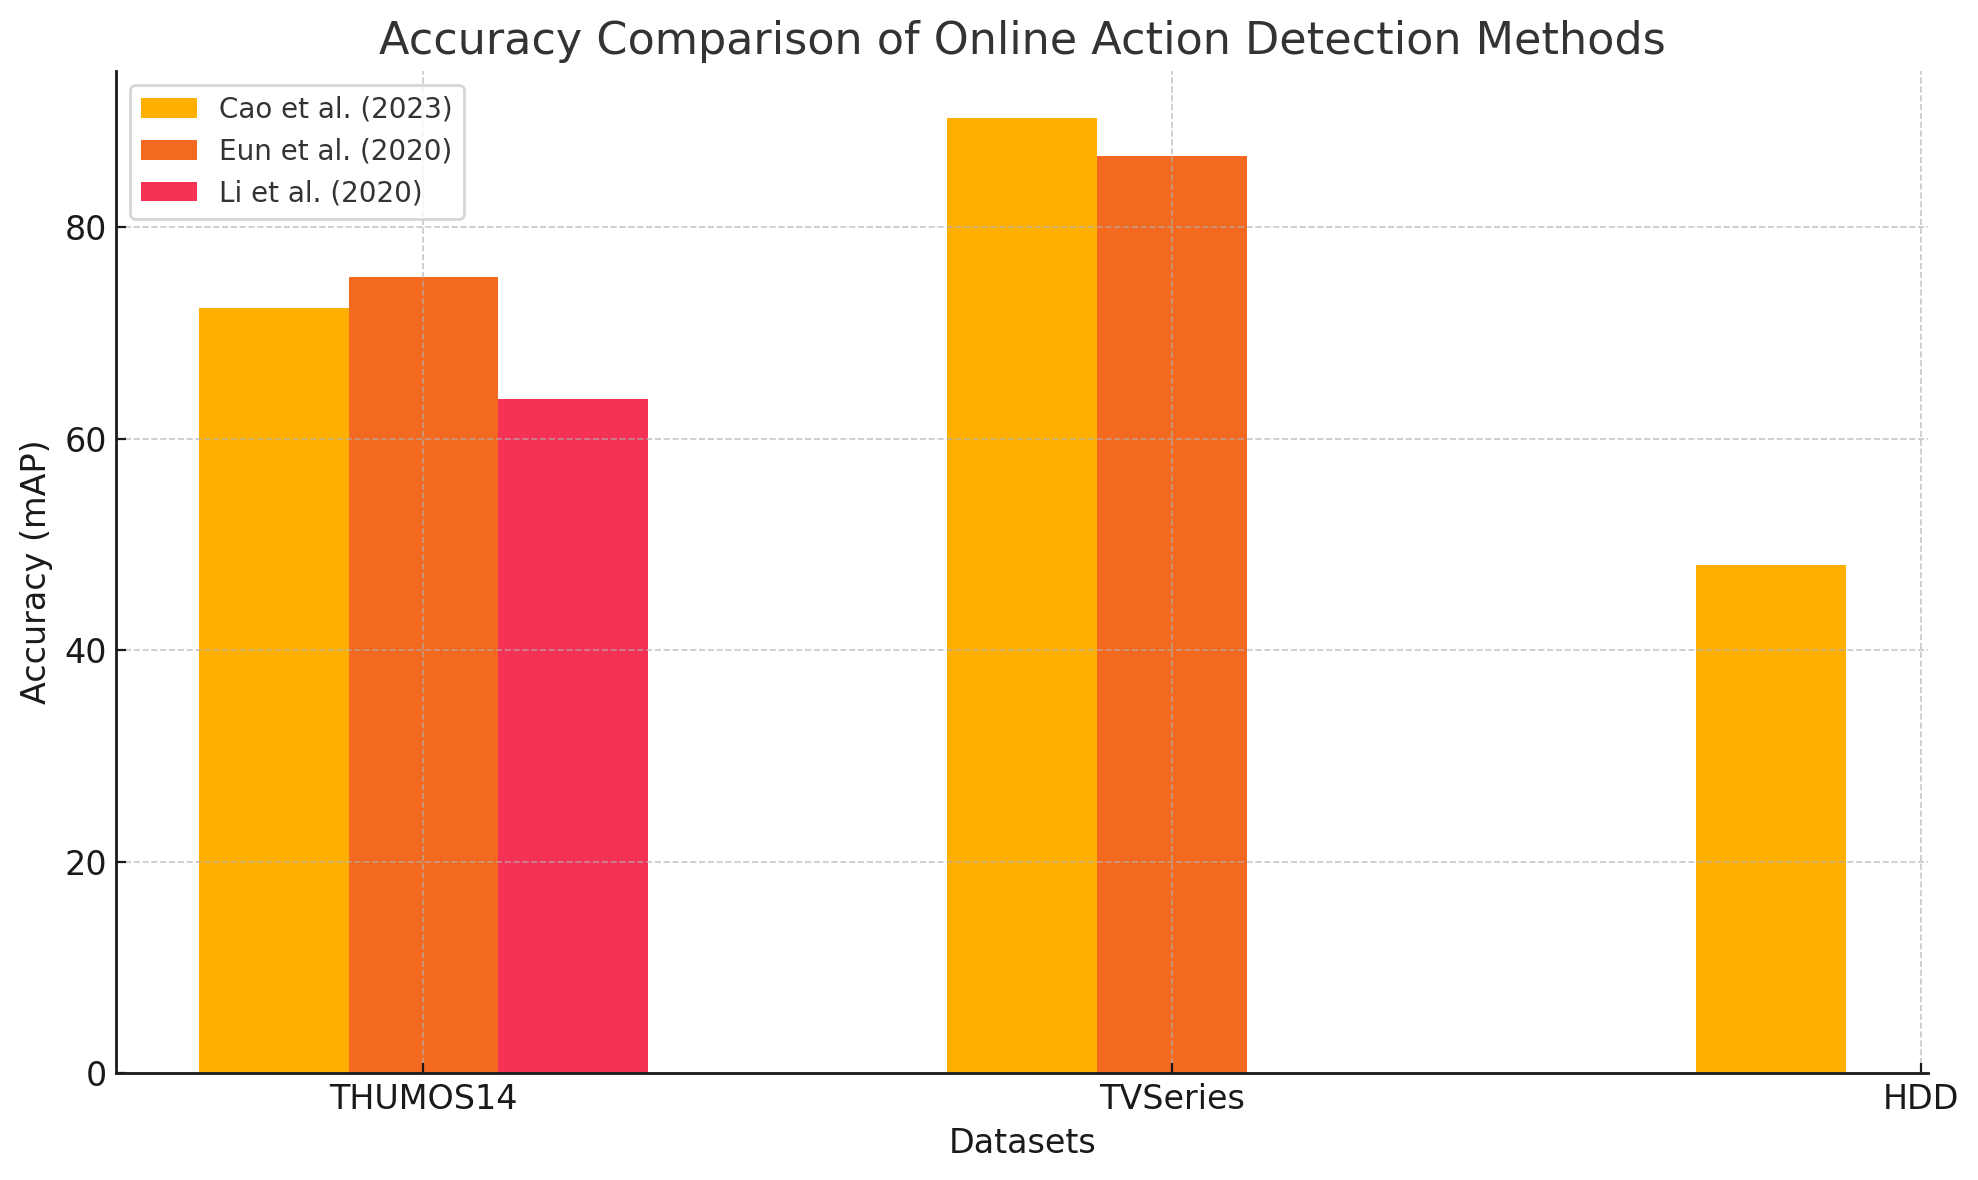
\includegraphics[width=5in]{img/acuracy.png}
    \caption{Accuracy Analysis}
    \label{fig:example}
\end{figure}

\section*{}
\begin{center}
    {\fontsize{14}{1.5}\selectfont \textbf{CHAPTER V}}\\
    \vspace{12pt}
    {\fontsize{16}{1.5}\selectfont \textbf{Comparison}}\\
    \vspace{12pt}
    \vspace{12pt}
\end{center}

\setcounter{section}{5}
\setcounter{subsection}{0}
\setcounter{table}{0}
\setcounter{figure}{0}
\addcontentsline{toc}{section}{\textbf{CHAPTER V Comparison}} % Add to ToC




{

\subsection{E2E-LOAD [ End-to-End Long-form Online Action Detection ]
}
E2E-LOAD introduces a thorough framework aimed at detecting actions in long, untrimmed videos. This method enhances the understanding of temporal context by using an e2e approach. It features temporal convolutional networks (TCNs) to capture temporal dependencies and integrates both spatial and temporal information to boost detection accuracy. By emphasizing long term dependencies  E2E-LOAD shows strong performance on benchmark datasets making it effective for complex real-world scenarios.

\subsection{IDN [ Information Discrimination Network ]
}
The Information Discrimination Network IDN improves the relevance of action detection features by incorporating an Information Discrimination Unit IDU. This unit enhances recurrent neural networks RNNs by filtering out irrelevant information from the input data allowing the network to focus on the ongoing action. The IDU employs current information and an early embedding module to maintain a discriminative representation of the action. IDN has demonstrated significant improvements over state of the art methods on benchmarks such as TVSeries and THUMOS14 effectively handling noisy and cluttered video streams.

\subsection{Methodology and Performance
}

E2E LOAD utilizes TCNs to capture long term dependencies and combines spatial and temporal data for precise action detection. Its e2e processing of long-form videos minimizes the need for extensive preprocessing. This method excels in scenarios that require detailed temporal context and has shown robustness across various datasets.
  
IDN enhances traditional RNNs with the IDU to filter out irrelevant information and emphasize current actions. This approach uses current input and early embedding to refine feature representation leading to more accurate detection. IDNs performance on the TVSeries and THUMOS14 datasets highlights its effectiveness in handling noisy input.

\subsection{Comparative Analysis
}

\subsubsection{Temporal Dependency Handling
}
E2E LOAD excels at capturing long term dependencies with TCNs  making it ideal for long continuous video streams where actions span extended periods.
IDN focuses on filtering relevant information and enhances RNN capabilities which are typically better for shorter temporal contexts compared to TCNs.

\subsubsection{Relevance of Features
}
E2E LOAD integrates spatial and temporal features without explicitly filtering irrelevant data.
IDN discriminates between relevant and irrelevant information using the IDU improving focus on current actions and reducing noise from irrelevant background activities.

\subsubsection{Benchmark Performance
}
E2E-LOAD demonstrates robust performance across various datasets due to its comprehensive temporal context handling.
IDN shows superior performance in noisy and cluttered environments with significant improvements on the TVSeries and THUMOS14 benchmarks.

\subsubsection{Implementation Complexity
}
E2E LOAD may be more complex to implement due to the integration of spatial and temporal data and management of long term dependencies.
IDN adds complexity through the IDU but remains relatively straightforward in enhancing RNN structures.

}
\section*{}
\begin{center}
    {\fontsize{14}{1.5}\selectfont \textbf{CHAPTER VI}}\\
    \vspace{12pt}
    {\fontsize{16}{1.5}\selectfont \textbf{Findings and Recommendations}}\\
    \vspace{12pt}
    \vspace{12pt}
\end{center}

\setcounter{section}{6}
\setcounter{subsection}{0}
\addcontentsline{toc}{section}{\textbf{CHAPTER VI Findings and Recommendations }} % Add to ToC

\subsection{Findings}{




\subsubsection{Enhanced Accuracy with Long-term History Integration:
}
   The E2E-LOAD model demonstrates that incorporating long-term historical data significantly boosts the accuracy of online action detection. This improvement is achieved through the Long-term Compression LC and Long-Short term Fusion LSF modules which integrate long-term historical data into short-term memory for better spatiotemporal modeling. By combining both long-term and short-term data the model achieves impressive performance metrics including a mean average precision mAP of 72.4 percent.

\subsubsection{ Efficiency Gains through Efficient Inference Technique:
}
   The Efficient Inference EI technique introduced in the E2E-LOAD model significantly enhances processing speed without sacrificing accuracy. By accelerating the spatiotemporal attention process the model achieves a substantial increase in frames per second FPS enhancing its real-time detection capabilities. For example incorporating EI increased the FPS from 9.1 to 19.5 in the baseline configuration demonstrating the techniques effectiveness in optimizing performance.

\subsubsection{Superior Accuracy with IDN Model:
}
   The Information Discrimination Network IDN surpasses existing state-of-the-art methods in online action detection by effectively distinguishing relevant information from irrelevant data. This ability allows the IDN model to achieve higher mean class accuracy performance mcAP with IDN-Kinetics reaching up to 86.1 percent mcAP. The models design reduces false detections by enhancing the discrimination of action-relevant information significantly contributing to its superior performance.

\subsubsection{Early Action Detection Capability:
}
   In online action detection identifying actions as early as possible is crucial. The IDN model excels in this aspect consistently maintaining high accuracy throughout action progression and showing significant improvements in early action detection segments compared to other models. This early detection capability is vital for real-time applications where prompt response to actions is necessary.

 
\subsection{Recommendations}

\subsubsection{ Integrate Long-term and Short-term Data:
}
 To enhance the performance of online action detection systems it is recommended to integrate long-term historical data with short-term memory. As demonstrated by the E2E-LOAD model this approach can significantly improve the accuracy of detecting ongoing actions. Implementing modules such as Long-term Compression LC and Long-Short-term Fusion LSF can provide a more comprehensive spatiotemporal context leading to better detection results.

\subsubsection{ Adopt Efficient Inference Techniques for Real-time Applications:
}
   Incorporating Efficient Inference EI techniques is crucial for applications requiring real-time action detection. By optimizing the spatiotemporal attention process these techniques can enhance processing speed and ensure timely detection without sacrificing accuracy. This is particularly important for systems deployed in dynamic environments where immediate action recognition is necessary.

\subsubsection{ Focus on Information Discrimination:
}
   Developing models that can effectively discriminate between relevant and irrelevant information is essential for improving detection accuracy. The success of the IDN model highlights the importance of enhancing information discrimination capabilities. Future models should incorporate mechanisms to filter out irrelevant data thereby reducing false positives and improving overall detection performance.

\subsubsection{Prioritize Early Detection Capabilities:
}
   Ensuring that models can accurately detect actions at the earliest stages is vital for many real-time applications. Enhancing early detection capabilities can lead to more responsive and proactive systems. It is recommended to design and train models with a focus on early action recognition possibly through specialized loss functions or training regimes that emphasize the importance of initial action segments.

By implementing these recommendations the development and deployment of online action detection systems can achieve higher accuracy efficiency and responsiveness effectively meeting the demands of real-world applications.

}


\vspace{12pt}
\vspace{12pt}
\vspace{12pt}

\begin{figure}[htbp]
    \centering
    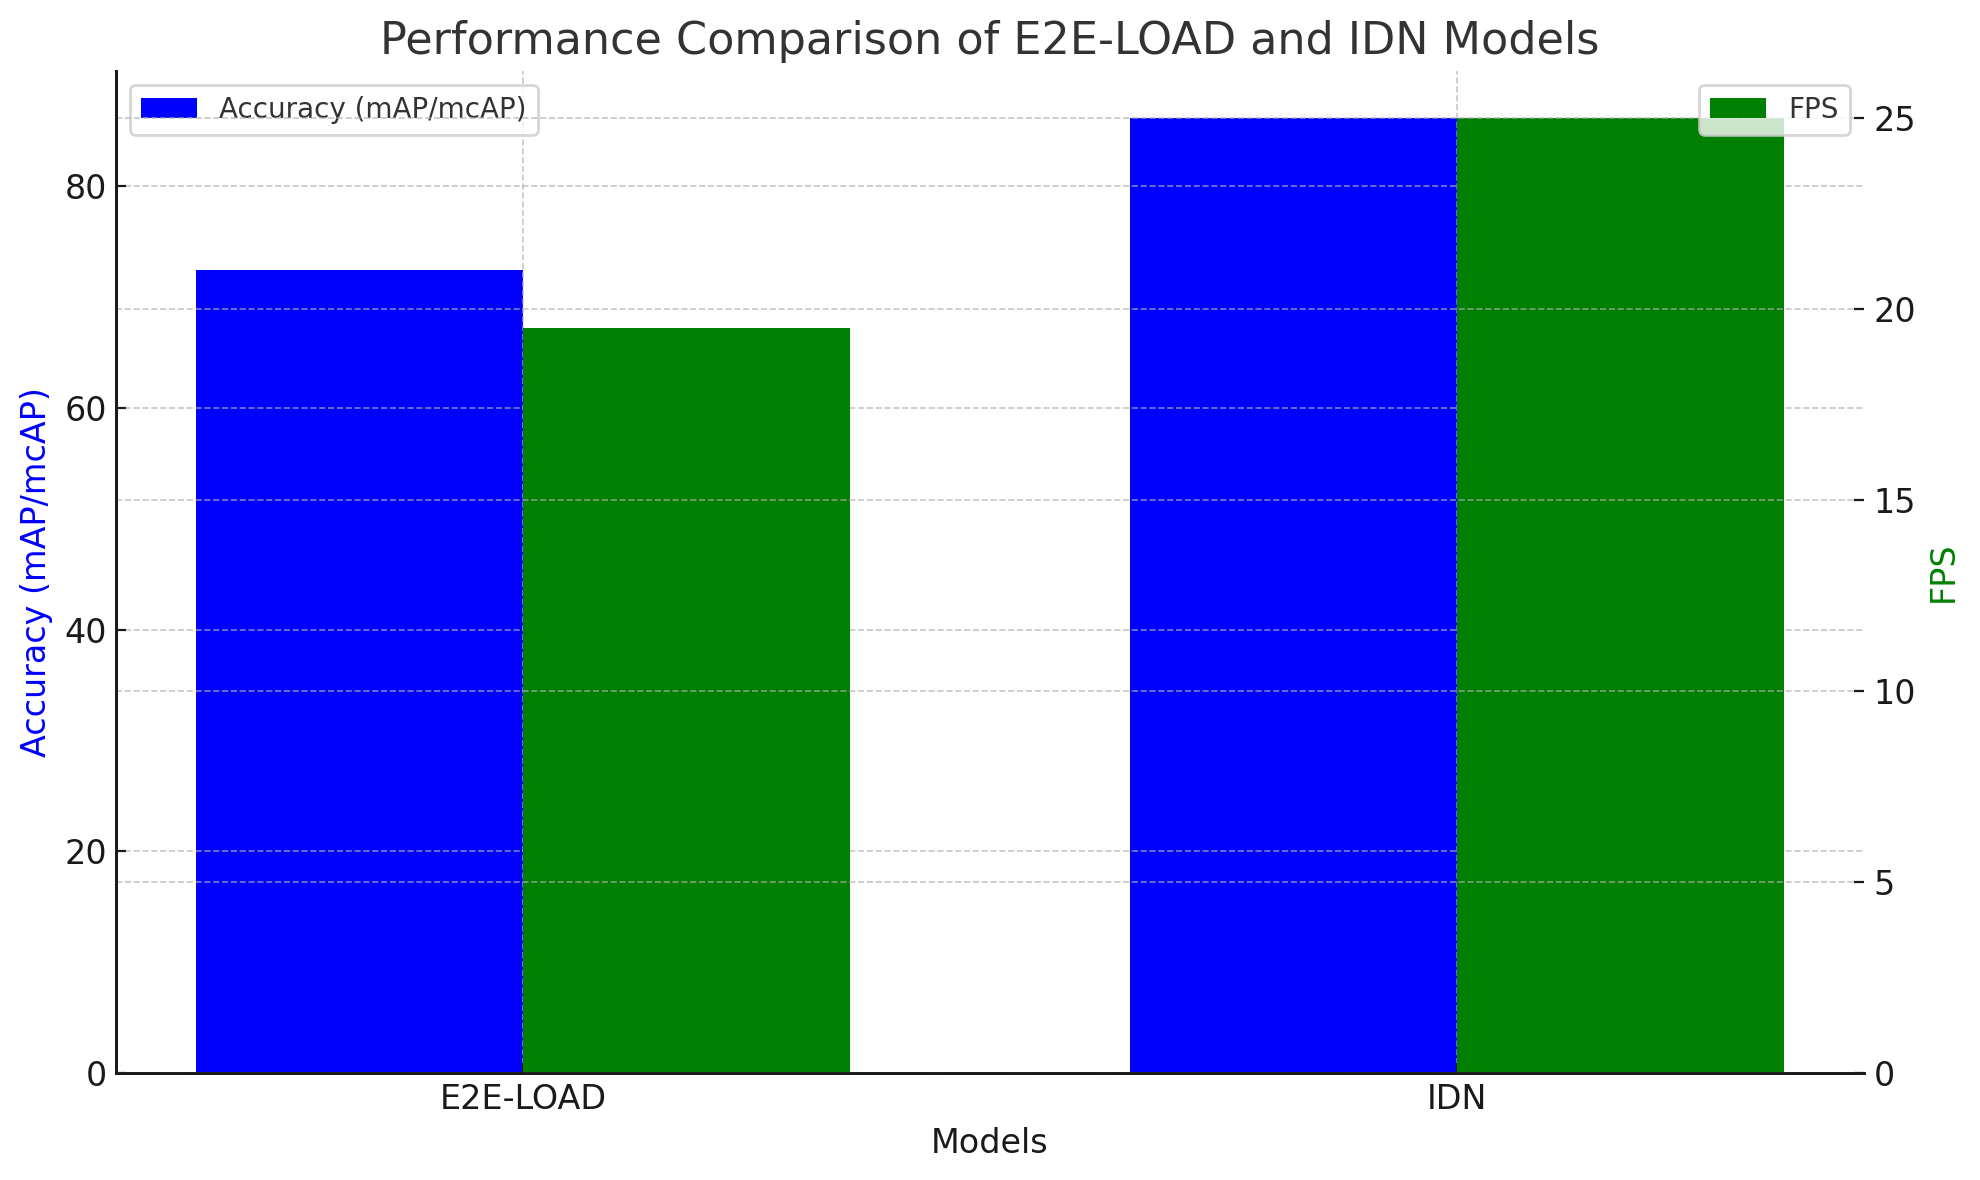
\includegraphics[width=6in]{img/performance.png}
    \caption{Performance Comparison}
    \label{fig:example}
\end{figure}

\section*{}
\begin{center}
    {\fontsize{14}{1.5}\selectfont \textbf{CHAPTER VII}}\\
    \vspace{12pt}
    {\fontsize{16}{1.5}\selectfont \textbf{Conclusions}}\\
    \vspace{12pt}
    \vspace{12pt}
\end{center}

\setcounter{section}{7}
\setcounter{subsection}{0}
\addcontentsline{toc}{section}{\textbf{CHAPTER VII Conclusions}} % Add to ToC

\subsection{Limitations} { 

High Complexity and Computational Demand  The E2ELOAD architecture is complex . It requires substantial computational resources for training  . It can be making  difficult for those with limited access to advanced computing systems to implement. The training process is both resource intensive and time consuming. 

Generalization challenges that the model shows strong performance on benchmark datasets.  It may struggle to generalize effectively to new unseen data and different contexts. This limitation is due to the training datasets which is encompassing the full range of variability .  It was found in real world scenarios which could affect the model's robustness.

Reliance on temporal Consistency  that the model's effectiveness depends heavily on the temporal consistency of actions within videos. Variations or interruptions in action sequences can negatively impact performance . It suggests a need for further refinement to handle such inconsistencies far better.

IDU - Information Discrimination Unit

Distinguishing background and irrelevant actions  the IDU model is built to differentiate between relevant and irrelevant information. However it can be challenging to accurately distinguish between background noise and subtle action cues in highly dynamic environments. It potentially leads to missed action details and misclassification of background activities .

Efficiency with long videos  the model's performance and accuracy can decline when processing extended video sequences. Maintaining temporal coherence and extracting relevant features over long periods is difficult for posing a challenge for the model's scalability.

Realtime processing limitations  implementing the IDU model in realtime applications can be problematic due to potential latency issues. Ensuring that the model processes incoming data streams quickly enough to provide . Timely action detection is crucial but remains a significant challenge.

Future frame generation FFG network for Online Action Detection

Limited backpropagation during training the training process is hindered by the inability to backpropagate errors effectively across the entire network due to resource constraints. Each component PR AR F2G is trained separately which can lead to suboptimal learning and integration as the final detection network's errors do not influence the entire system.

Dependence on Generated Frames: The performance of the FFG network is dependent on the quality of the generated future frames. If these generated frames are not accurate enough the overall detection performance can suffer. Current methods for frame generation still need to improve to match the realism and accuracy of actual frames.

\subsection{Disscussion}
Computational intensity in the framework's reliance on multiple deep networks . It constructs a sliding window approach results in high computational demands. This complexity poses challenges for realtime deployment. It  may not be feasible on standard hardware without significant optimizations

Handling High IntraClass Variation: Recognizing actions with high intra class variability remains a challenge. While decomposing actions into beginning and finishing phases helps it does not fully address the issue of reliably detecting highly variable actions.

Advancements in online action detection as illustrated by models like E2ELOAD and the Information Discrimination Network IDN mark substantial progress in the domain. These model introduced distinct strength and innovative solutions. It can tackle the challenges of realtime action detection.
\subsection{Conclusion}
E2ELOAD leverages temporal convolutional networks TCNs to effectively capture long term dependencies combining spatial and temporal information to boost detection accuracy. This method is particularly advantageous for analyzing longform videos where actions extend over considerable periods. Despite its complexity and high computational demands  for E2ELOAD . It demonstrates strong performance across various datasets. It is proving its capability in managing complex real world scenarios.

IDN introduces the Information Discrimination Unit IDU to enhance feature relevance by filtering out irrelevant data. By improving recurrent neural networks RNNs this model focuses more precisely on ongoing actions significantly boosting detection accuracy in noisy and cluttered environments. IDN's strength lies in managing irrelevant information and maintaining high accuracy in early action detection making it highly effective for realtime applications.

However both models have limitations. E2ELOAD’s complexity and significant computational requirements may limit its accessibility . Its dependency on temporal consistency can impact performances .  Meanwhile IDN though adept at filtering relevant information can struggle . It is distinguishing subtle action cues in dynamic environments .

Future research should focus on enhancing computational efficiency.  It  is improving generalization capabilities and refining techniques. It is for managing variability and inconsistencies in action sequences . Addressing these challenges will help develop more robust efficient and accurate models.  It is  for a broader range of real world applications.

In conclusion E2ELOAD , IDN each significantly advance online action detection. Their innovative approaches and proven effectiveness in various contexts highlight their potential. It is used  to meet the demands of realtime dynamic environments . It is paving the way for future improvements and applications in the field.}
\section*{}
\begin{center}
    {\fontsize{14}{1.5}\selectfont \textbf{CHAPTER VIII}}\\
    \vspace{12pt}
    {\fontsize{16}{1.5}\selectfont \textbf{Publication Details
}}\\
    \vspace{12pt}
    \vspace{12pt}
\end{center}
\setcounter{section}{8}
\setcounter{subsection}{0}
\addcontentsline{toc}{section}{\textbf{CHAPTER VIII Publication Details
}} % Add to ToC
\renewcommand{\theequation}{\thesection.\arabic{equation}}
\renewcommand{\thetable}{\thesection.\arabic{table}}
\renewcommand{\thefigure}{\thesection.\arabic{figure}}
\setcounter{table}{0}
\setcounter{figure}{0}
\setcounter{equation}{0}

\begin{figure}[htbp]
    \centering
    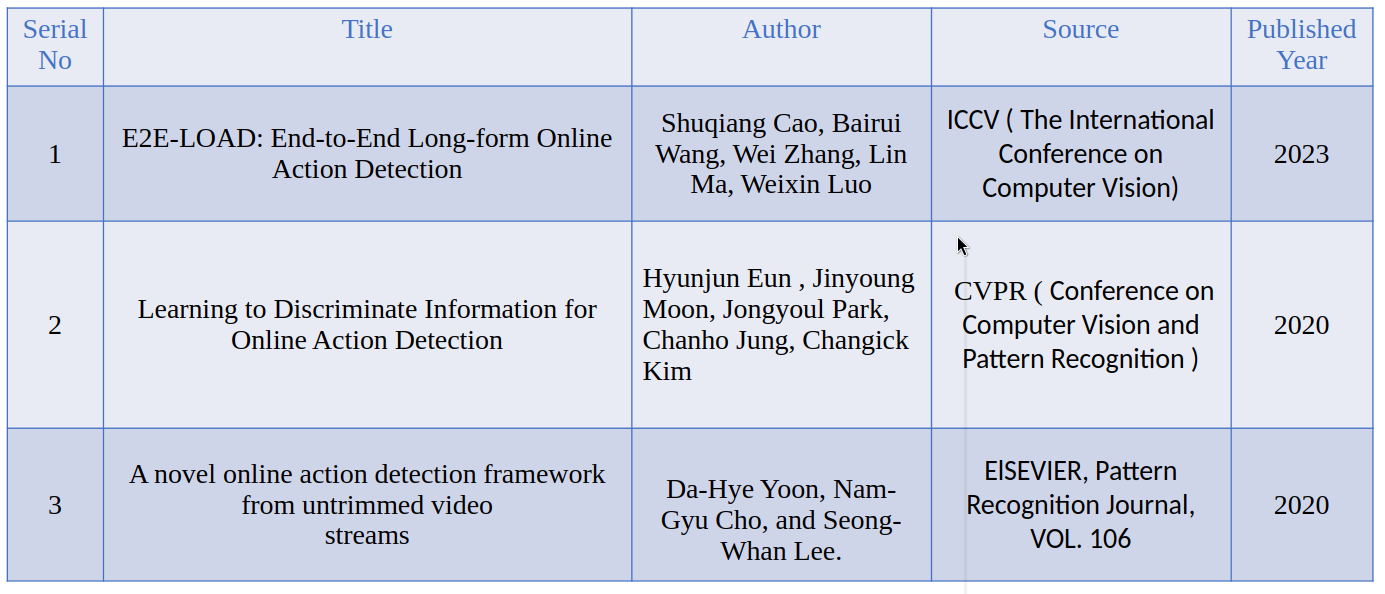
\includegraphics[width=6.5in]{img/publication.png}
    \caption{Paper Information}
    \label{fig:example}
\end{figure}



\addcontentsline{toc}{section}{\newline References} % Add to ToC

\renewcommand\bibname{References}
\bibliographystyle{unsrt}   
\bibliography{references}

\phantom {
\cite{0}
\cite{1}
\cite{2}
\cite{3}
\cite{4}
\cite{5}
\cite{6}
\cite{7}
\cite{8}
\cite{9}
}
\end{document}

